
%\renewcommand{\familydefault}{\sfdefault}
%=============== En−Tete ===============
 
%−−− Insertion de paquetages −−−−
\documentclass[12pt,a4paper]{report}
\usepackage[utf8]{inputenc}
\usepackage{amsmath}
\usepackage{amsfonts}
\usepackage{amssymb}
\usepackage{graphicx}
\usepackage{wrapfig}
\graphicspath{ {./images/} }
\usepackage[rightcaption]{sidecap}
\usepackage{subcaption}

\usepackage[french]{babel}
\usepackage[Sonny]{fncychap}
\usepackage{fancyhdr}
\usepackage{float}
\usepackage{epsfig}
\usepackage{appendix}
\usepackage[final]{pdfpages}
\usepackage{array}
\usepackage{pdfpages}

\pagestyle{fancy}


%−−− Page de garde - titre −−−

\begin{document}

\title{\Large{\textbf{Skip List \vskip3pt \Large Travail de lecture et de rédaction scientifique sur le Federate Learning}}}

\author{Bal Sébastien}

\maketitle

\thispagestyle{empty} % Ignore page number


 

%=============== Remerciement ===============

\begin{figure}[p]

\large\textbf{Remerciements}

\end{figure}


 

\thispagestyle{plain}\setcounter{page}{1} % Start page count


 

\fancyhead[LE,RO]{\leftmark}

\fancyhead[RE,LO]{}

\fancyfoot[R]{\textbf{\thepage}}

\fancyfoot[C]{Master en Science infomatique - Lecture et rédaction scientifique}


 

\tableofcontents

\chapter{Machine Learning}

Le Machine Learning est une sciences moderne qui permet d'effectuer des prédictions à partir de données qui se basent sur des statistiques. \\

Cette méthode fait partie d'une branche de l'intelligence artificielle qui englobe plusieurs méthodes afin de créer automatiquement des modèles à partir de données. \\

Le Machine Learning prend de l'expérience au fur et à mesure que l'algoithme est exposé à davantages de données. C'est ainsi que celui ci permet de s'améliorer. Un programme informatique quand à lui, ne fait que suivre des instructions précises.\\

Le Machine Learning peut etre différencié par deux types d'algorithmes : supervisés et non supervisés.L'apprentissage supervisé utilise des données qui sont déjà connues par le model avec une étiquette. A la fin de son entrainement,le model pourra être capable de retrouver des données dans le même domaine dont les données n'ont pas d'étiquette.\\


\begin{center}
	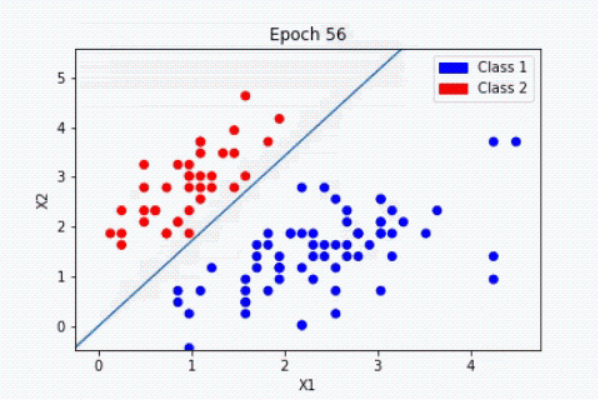
\includegraphics[scale=0.4]{machine_learing_1}
	\captionof{figure}{Modèle supervisé}
	\label{fig1}
\end{center}


Sur cette image ci dessus, on peut constater que l'algorithme ajustera sont modèles en fonction de ses paramètres afin de diminuer l'écart entre les résultats attendus et les résultats obtenus. Ce qui diminuera au fil de l'entraînement les marges d'erreurs. \\

L'apprentissage non supervisé, quand à lui, permet d'entrainer le modèle sans étiquette. La machine cherche parmis les données sans indices et permet de découvrir les tendances.L'apprentissage par renforcement, ce modèle permet d'entrainer la machine avec un objectif bien précis.Le modèle a un système d'échecs et d'erreurs. \\






\section{En quoi consiste le Machine Learning}

Le Machine Learning est présent partout sur la toile, cela va au moteur de recherche comme Google. Nos applications tels que Siri et Alexa. Les fils d'actualités comme Facebook et Twitter. Toutes ces platformes stockent des données sur les utilisateurs afin de comprendre et d'améliorer leurs performances. Ces données serviront à mieux cibler ce que les utilisateurs aiment. La machine pourra ainsi proposer plus facilement des recommandations ou des résultats pour des recherches.
\pagebreak


\section{Big Data et Machine Learning}

Avec un grand nombre de données les outils analytiques ne savent pas traiter autant de donnés pour l'exploiter à bon escient. Un volume de données trop large empèche une analyse compréhensive. Les corrélations et les relations entre ces données sont trop importantes ce qui complique la tache pour des analystes. 

C'est pour cette raison que le Machine Learning est idéal pour du Big Data. Cette technologie pourra extraire des valeurs qui proviennent de cette source de données sans passer par l'intermèdiaire d'un être humain.

Sans le Big Data, le Machine learning et l'intelligence artificielle ne sont rien. Les données sont le moyen pour le Machine Learning d'apprendre et de comprendre comment pensent les humains. 

La technologie est capable d'apprendre en allant chercher elle même des ensembles de données pour les analyser et devenir plus précise.

\section{Deep Learning, sous domaine du Machine Learning}

Le Deeo Learning est basé sur un système d'un réseau neuronal inspiré des systèmes cérébraux. Ce type d'apprentissage est d'y supervisé car c'est le développeur qui va décidé sur quel type d'apprentissage il va lancer le Deep Learning. Cette technique à besoin d'énormément de données, on parlera donc de Data Lake. 

Pour que le modèle mathématique deviennent performant, il faudra l'entrainer à reconnaitre un élément en particulier. Prenons le cas de la reconnaissance d'un animal. Pour la phase d'apprentissage nous passerons au système plusieurs images d'animaux. On précisera dans la partie d'entrainement les éléments auquels le système devra être conscient.
\pagebreak

Pour notre exemple, les boules vertes représente le bon chemin que le système va prendre pour arriver à vérifier le modèle qui était demandé. Les boules bleus sont celles qui ont des caractéristiques avec le modèle mais ne correspondra pas exactement au modèle qui était demandé. Les boules rouges quand à elles, représentent les erreurs que le système a exclu pour pouvoir apprendre le modèle exacte. Les erreurs sont par la suite renvoyées en amont du système pour que le système ajuste son modèle mathématique

\begin{center}
	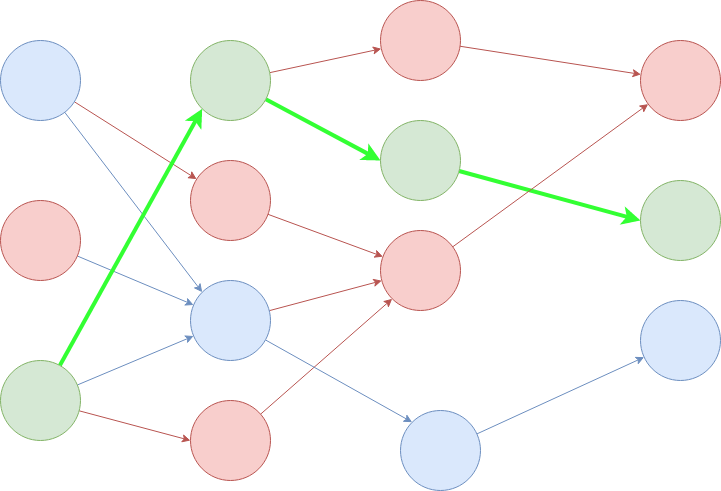
\includegraphics[scale=0.4]{deep_learning_schema}
	\captionof{figure}{Autoapprentissage Deep Learning}
	\label{fig1}
\end{center}

\chapter{Federate Learning}
\section{Le Federate Learning c'est quoi ?}

En quelques mots, c'est un apprentissage automatique distribué qui permet d'entraîner un modèle mathématique avec un large groupe de données décentralisées qui se trouvent sur des téléphones portables(pour notre cas ici).

\section{TensorFlow explication}
Dans notre modèle, nous allons utilisé le système TensorFlow pour former notre système neuronal. TensorFlow est une bibliothèque open source pour le Machine Learning. C'est un petit couteau Suisse qui contient ici des outils pour permettre de résoudre des problèmes mathématiques. 



\begin{thebibliography}{9}

	\bibitem{lamport94}
	  Leslie Lamport,
	  \emph{\LaTeX: A Document Preparation System}.
	  Addison Wesley, Massachusetts,
	  2nd Edition,
	  1994.
	  
	\bibitem{bigdata}
	Pour la partie sur le Machine Learning https://www.lebigdata.fr/machine-learning-et-big-data

\end{thebibliography}


\label{Pour la partie sur le Machine Learning https://www.lebigdata.fr/machine-learning-et-big-data}

\label{TensorFlow : https://www.lebigdata.fr/tensorflow-definition-tout-savoir}

%Citeseer citeseer.ist.psu.edu,Google Scholar scholar.google.com,ScienceDirect www.sciencedirect.com,ACM Digital Library portal.acm.org,IEEE Digital Library www.computer.org/portal/site/csdl/index.jsp


\label{https://www.youtube.com/watch?v=QR1SnCRungE&ab_channel=AlainOlivetti} 


\begin{appendix}
 \chapter{Annexe}
 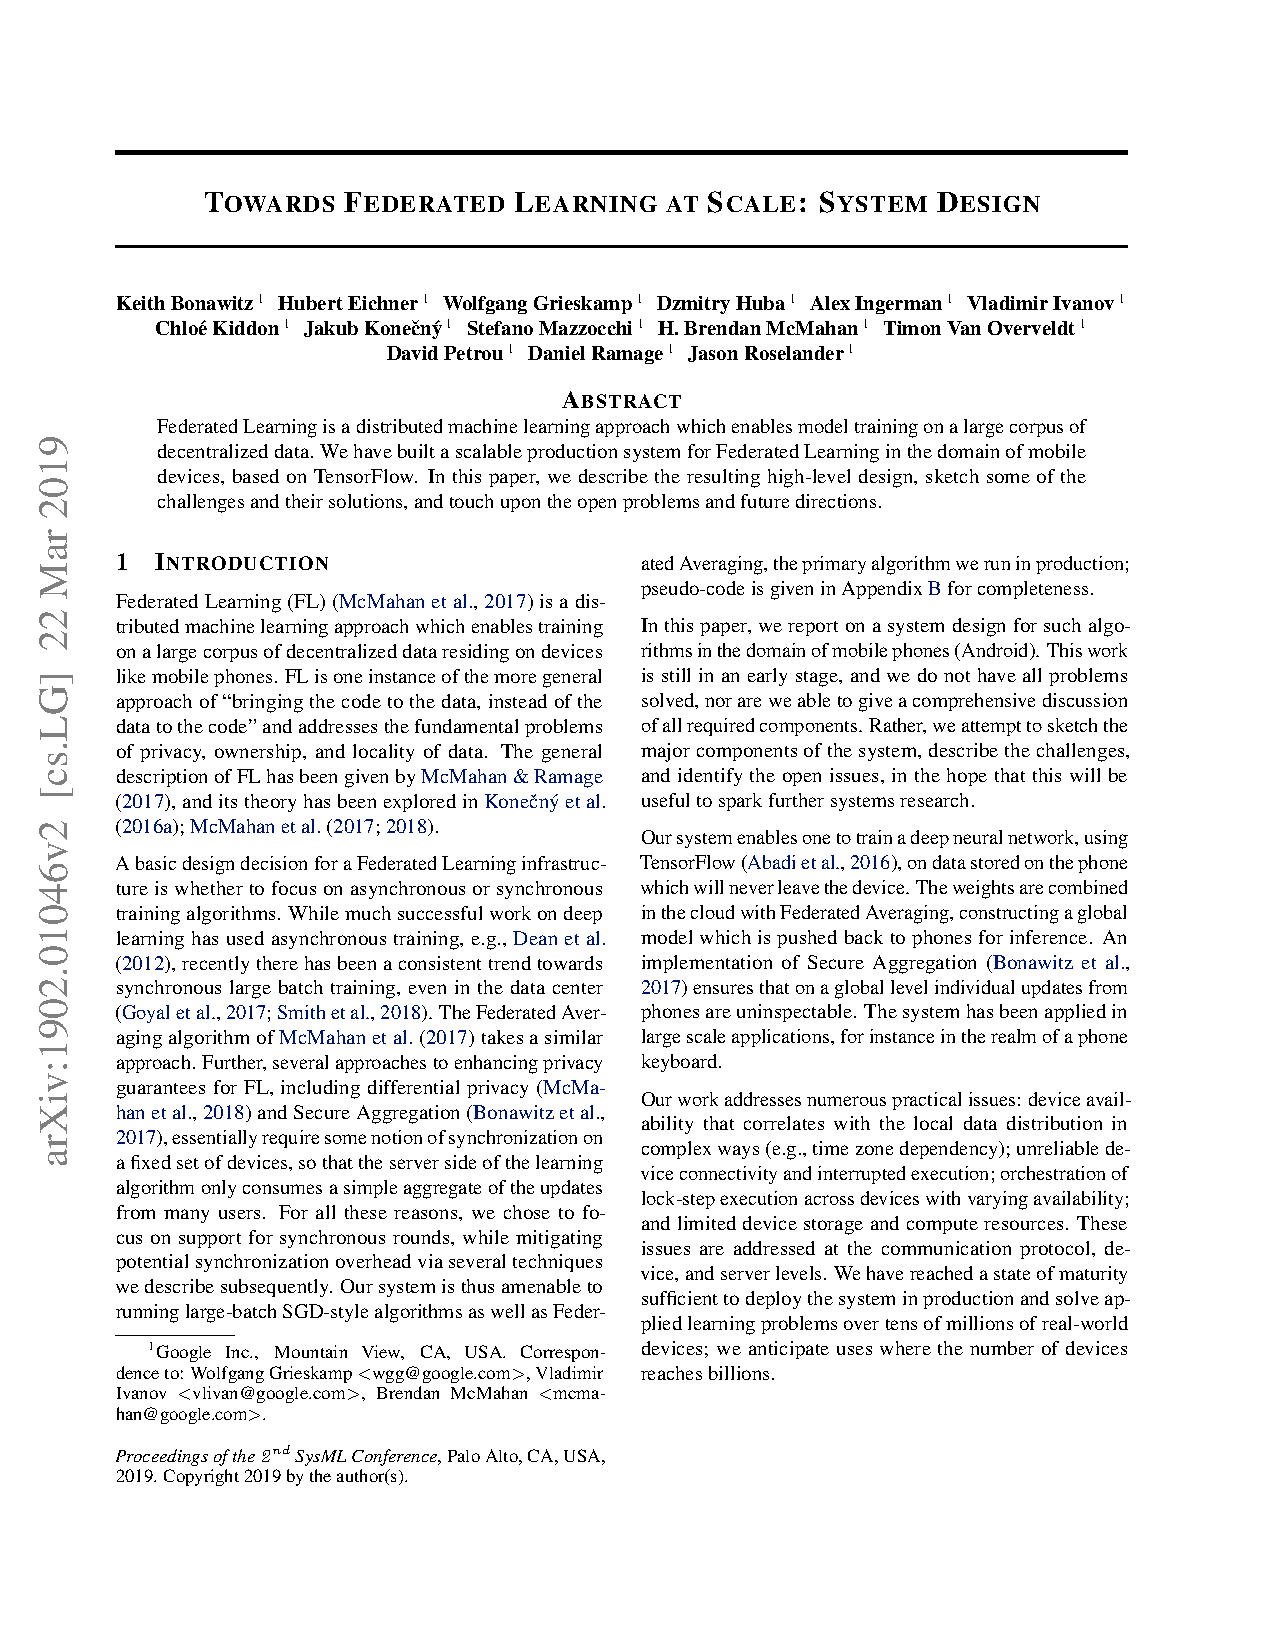
\includepdf{pdf/federate_learning_en.pdf}
\end{appendix}

\end{document}
